\section{Experiments}

\subsection{Monk Results}

\subsubsection{Architecture and hyper-parameters}
For all MONK problems, we adopt one-hot encoding for representing the inputs, so we use neural networks with $17$ input units. We use $1$ hidden layer with $4$ units for the first two problems and $15$ for the last one. About activation functions, we use \texttt{tanh} for the hidden layer, and \texttt{sigmoid} for the output layer to get outputs in the $[0, 1]$ range.

We choose \texttt{MSE} as the loss function over the "raw" output of the \texttt{sigmoid} in order to have differentiability, and instead for predictions every input is classified as $1$ if the output of the \texttt{sigmoid} is $\ge 0.5$ and $0$ otherwise.

We use mini-batch gradient descent with $\texttt{batch\_size}=2$ for all Monk problems, and L2 regularization with parameter $\lambda$ for Monk3.

Our choice of hyper-parameters is shown in \cref{fig:hyper} below, along with the performance averaged over $5$ different runs to avoid the bias due to weights initialization.

\begin{figure}[h]
    \centering
    \begin{tabular}{|l|c|c|c|c|}
        \hline 
        Task & $\eta$ & $\lambda$ & Loss (train/test) & Accuracy (train/test) \\ \hline
        MONK 1 & 0.5 & 0 & 0.00039/0.00047  & 100\%/100\% \\ \hline
        MONK 2 & 0.1 & 0 & 0.00223/0.00261 & 100\%/100\% \\ \hline
        MONK 3 & 0.01 & $10^{-5}$ & 0.06075/0.04557 & 93.44\%/97.22\% \\ \hline
    \end{tabular}
    \caption{Performance results on MONK datasets}
    \label{fig:hyper}
\end{figure}

\begin{figure}
    \centering
    \subfloat[Loss]{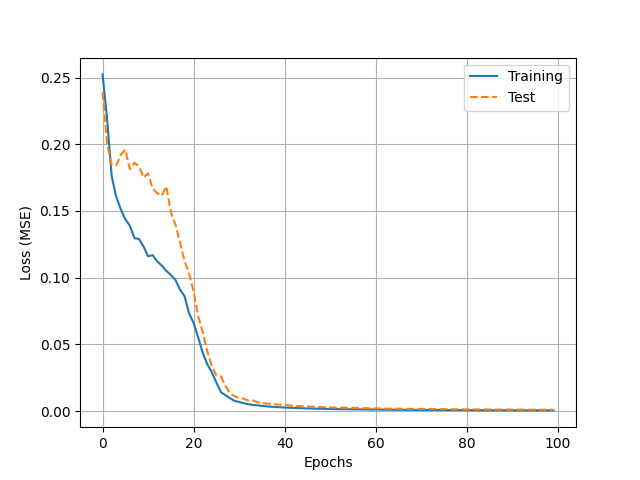
\includegraphics[width=0.5\textwidth]{../results/monks/monk1_losses.png}}
    \subfloat[Accuracy]{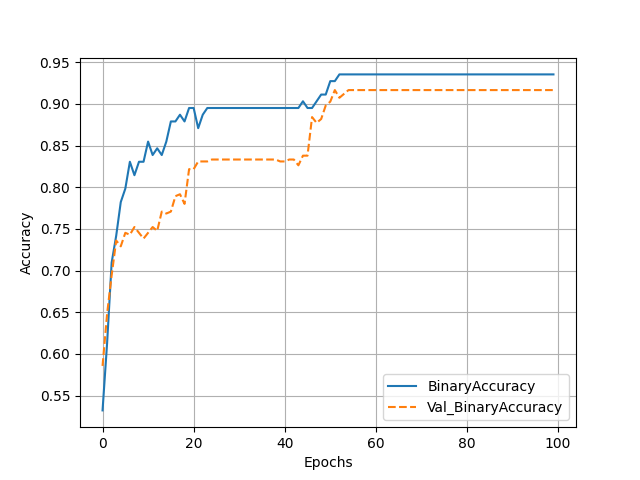
\includegraphics[width=0.5\textwidth]{../results/monks/monk1_accuracy.png}}
    \caption{Loss and accuracy of MONK 1}
    \label{fig:monk1}
\end{figure}

\begin{figure}
    \centering
    \subfloat[Loss]{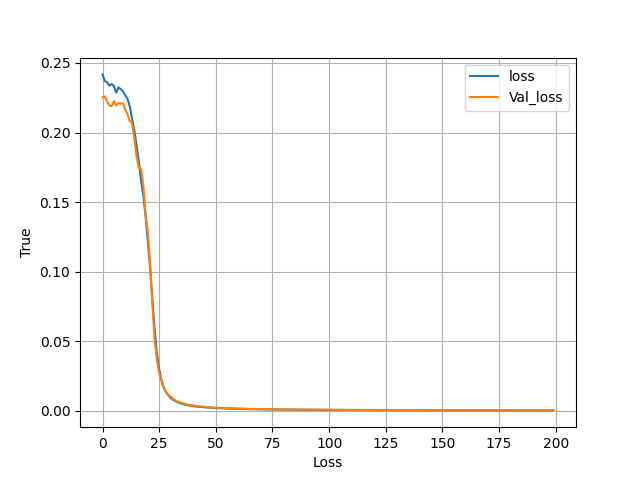
\includegraphics[width=0.5\textwidth]{../results/monks/monk2_losses.png}}
    \subfloat[Accuracy]{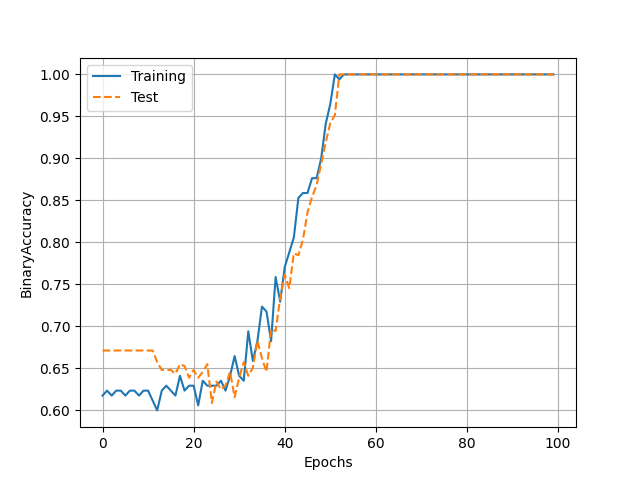
\includegraphics[width=0.5\textwidth]{../results/monks/monk2_accuracy.png}}
    \caption{Loss and accuracy of MONK 2}
    \label{fig:monk2}
\end{figure}

\begin{figure}
    \centering
    \subfloat[Loss]{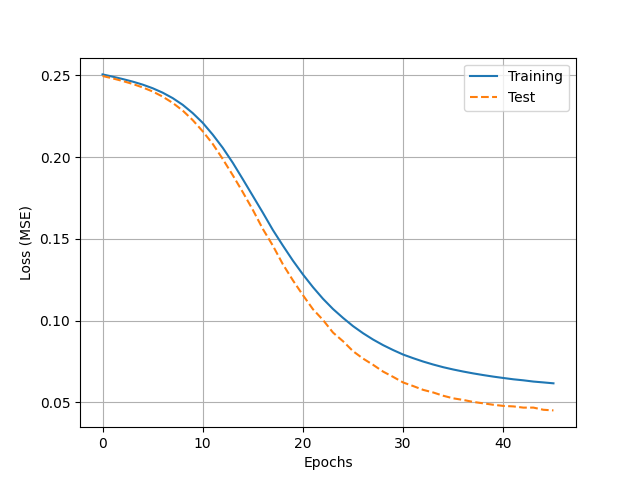
\includegraphics[width=0.5\textwidth]{../results/monks/monk3_losses.png}}
    \subfloat[Accuracy]{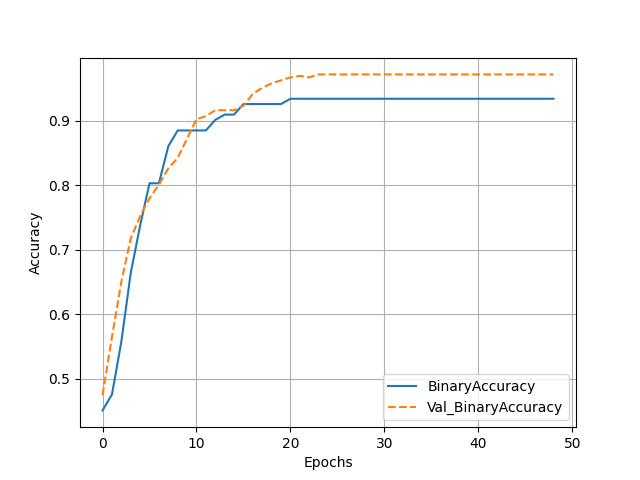
\includegraphics[width=0.5\textwidth]{../results/monks/monk3_accuracy.png}}
    \caption{Loss and accuracy of MONK 3}
    \label{fig:monk3}
\end{figure}

\subsection{CUP results}

We split the CUP dataset in \textbf{Development Set} ($90\%$ of the dataset, $1343$ records) and in  \textbf{Internal Test Set ($10\%$ of the dataset, $149$ records)}. The aim of the first dataset was to be used for subsequent train-validation splits for model selection and training, while the second one was used for testing. 

% questa cosa va davvero detta? dove?
 * before training and at the end of each epoch we shuffled the current training dataset

 The metric used for evaluation is MEE.

\subsubsection{Preliminary trials}

Before starting the grid search we decided to run some test with early stopping, splitting the development set in train set ($75\%$) and validation set ($25\%$). 

It revealed us that in most cases before epoch $1000$ the improvement on training set was of order of $10^-4$, while the loss on the validation set started to grow. Since we wanted to use also K-fold for model selection, and so we would not have a validation set for using early stopping, we decided to put $500$ as the maximum number of epoch to limit possible overfitting.

We similarly ran other test to discard some parameters and speed up the grid search. 

This led us to discard learning rates of $10^-1$ and $10^-4$, since they showed worse results than $10^-2$ and $10^-3$, and to select a batch size of $64$ or $32$, which consistently provided smoother learning curves than $8$ and $16$ without a loss in performance. 

We also tested different network architectures, and we noticed that the ones with two hidden layers performed better then the ones with a single hidden layer. The ones with three hidden layers performed no better then the former, so we understood that 2 was the ideal number of hidden layers.
In particular we considered architectures with at most $16$ units per layer, since we observed that for higher values performance started to worsen.


Finally, we discarded small values for weights initialization (e.g. uniform distribution in $[-0.1, 0.1]$), since they performed worse than higher ranges, for example ($[-0.5, 0.5]$).
Instead we adopted "fan-out" initialization to adapt the range of possible values to the number of units per layer.

\subsubsection{Grid search}

We developed two successive searches:
\begin{itemize}
    \item The first is an exhaustive Grid Search over a grid of $4320$ configurations, for which we used an Holdout validation strategy with the same split of the preliminary trials;
    
    \item The second is a sequential search among the models that best scored after the grid search, for which we used a 5-fold cross validation strategy.
\end{itemize}

The grid search was performed exhaustively among the following parameters:

\begin{itemize}
    \item Architecture (hidden units): 16-16, 16-8, 8-8;
    \item Activation functions (for hidden layers): tanh-tanh, tanh-sigmoid, sigmoid-tanh, sigmoid-sigmoid;
    \item (Initial) learning rate ($\eta_0$): 0.01, 0.005, 0.001;
    \item Momentum: 0, 0.2, 0.4, 0.6, 0.8;
    \item L2 Regularization Lambda: $10^{-6}$, $10^{-7}$;
    \item Minibatch size: 32, 64;
    \item Learning Rate Decay: no decay, linear decay up to $0.1 \cdot \eta_0$, linear decay up to $0.01 \cdot \eta_0$;
\end{itemize}

where with "linear decay up to $\eta_1$" we mean that if the number of epochs is $N$ (in our case $N = 500$), at the epoch $0 \leq x \le N$ (counting from $0$) we had a learning rate of $\eta(x) := \left(1 - \frac{x}{N}\right)\eta_0 + \frac{x}{N} \eta_1$. We have used a "relative" value of $\frac{\eta_0}{\eta_1}$ rather than a fixed constant $\eta_1$ in order to be sure that it always holds $\eta_1 \leq \eta_0$ (otherwise we could have got $\eta_0 = \eta_1 = 10^{-3}$ for instance).

After that first search, we ranked all the configurations according to their final validation MEE and we picked up the best $25\%$ configurations. We then performed a \textbf{5-fold cross validation} on all of them and we ranked them again according to their average final validation MEE over all the folds. 
 
The aim of this technique is to try to have a first "screening" search on a high number of combinations in order to do a deeper search (using 5-fold validation) on a set of configurations that we know already performed quite well in a training cycle. By keeping $25\%$ of the original models we managed to maintain a sufficiently wide range in terms of minimum and maximum MEE on the first search to limit the bias that the original train-validation split produces.

Finally, we selected the best model as our final model, trained it on the whole development set and used it for predicting outputs for the blind test set.

% qua magari scriviamo delle cose più precise (ma c'è una sezione più avanti per le specifiche dei pc)
The whole process took 6 hours of computation overall, deploying all 16 CPUs of Salvatore's PC.

% secondo lui ci vorrebbe una tabella di risultati della grid search, ma mi sembra irrealistico

 The best model is then trained on the whole development set and used for predicting outputs for the blind test set.

\subsubsection{Chosen model}

% dobbiamo inventarci delle osservazioni intelligenti?

As a result of the grid search our best model has a topology of 9-16-8-2 with \texttt{tanh} activations. Hyperparameters are $\eta=0.01,\lambda=10^{-7}$, without momentum, with minibatch size of $32$ and linear decay of $0.01$.

%  quello che sto per dire non è vero, questo è sul validation set. dove sono i risultati del blind test
We achieved an average MEE of $1.434$ on our blind test %, taken as an average of 10 different trainings of type A networks (to avoid the bias due to the random weight initialization). (abbiamo fatto così noi?)

We can see the learning curve of one of them in \cref{fig:typeA} below.

\begin{figure}[h]
    \centering
    \subfloat[Loss\label{fig:cup_loss}]{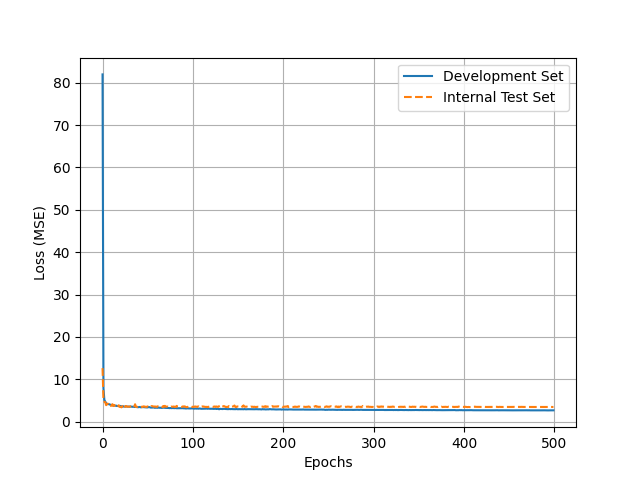
\includegraphics[width=0.55\textwidth]{../results/cup_loss.png}}
    \subfloat[MEE\label{fig:cup_MEE}]{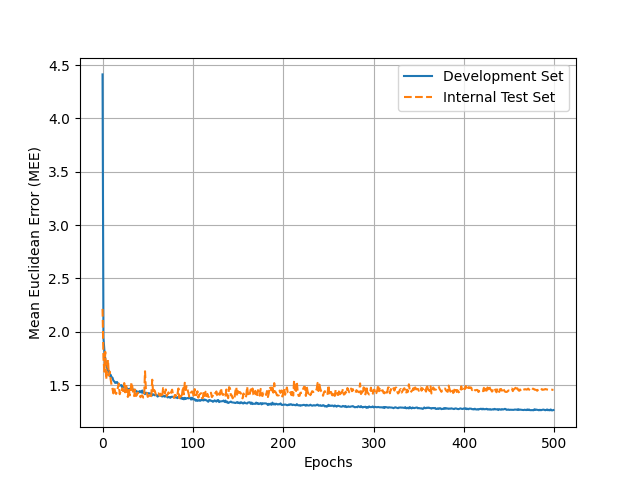
\includegraphics[width=0.55\textwidth]{../results/cup_MEE.png}}
    \caption{Learning curves for CUP network}
\end{figure}

%Then we tried an \emph{ensemble} approach: we trained 20 networks of type A and regarded the output of our model as the average of the outputs of the 10 bests (over validation benchmark) trained networks. (non l'abbiamo fatto, vero?)

%In this way we achieved a MEE error on the internal test set of $1.085$.

\begin{figure}
    \centering
    \begin{tabular}{|l|l|l|l|}
        \hline
        id & Train MEE & Valid MEE & Test MEE \\ \hline
        1 & 1.271 & 1.434 & non so \\ \hline
    \end{tabular}
    \caption{MEE of our NN}
    \label{fig:cup55-table}
\end{figure}
 % dove sono i risultati? 



%%% Local Variables:
%%% mode: latex
%%% TeX-master: "report"
%%% End: